
\documentclass{article}
\usepackage{amsmath}
\usepackage{graphicx}
\usepackage{multirow}
\usepackage{natbib}
\usepackage{caption}
\usepackage[margin=1in]{geometry}
\begin{document}
        
\title{Credit Balance MLR}


\author{Greg Sadler and Jackson Curtis}
\maketitle 

\section{Introduction}

One of the ways credit card companies make money is by credit card users accruing interest on their monthly balance. However, users who run high balances frequently face bankruptcy which results in a significant loss to the credit card company because they have to write off the balance. Therefore, the credit company's ideal customers carry a medium balance with low risk of bankruptcy. 

Because of this, credit card companies are interested in being able to estimate the balance a customer will carry based off other information they have on the customer. This estimate could be used predictively in the credit card approval process (where customers are given cards only if they are likely to be a profitable customer) or descriptively (where the company uses what they learn about customers with medium balances to target advertising towards people with those same characteristics). Our analysis will address both these questions.

The dataset we have been given contains the monthly balance of customers, along with ten explanatory variables. We will learn about the explanatory variables by performing multiple linear regression with balance as our response variable. This will allow us to obtain estimates for the effects of the explanatory variables, predictions for future observations, and uncertainty estimates for both.

\section{Data Exploration}
We'll start by exploring the data we have been given and make sure that it meets the assumptions of multiple linear regression. The data set consists of 294 individuals with 11 observed variables and no missing data. Four variables (gender, ethnicity, marital status, and student status) are categorical while the rest are quantitative.
\begin{figure}
\centering
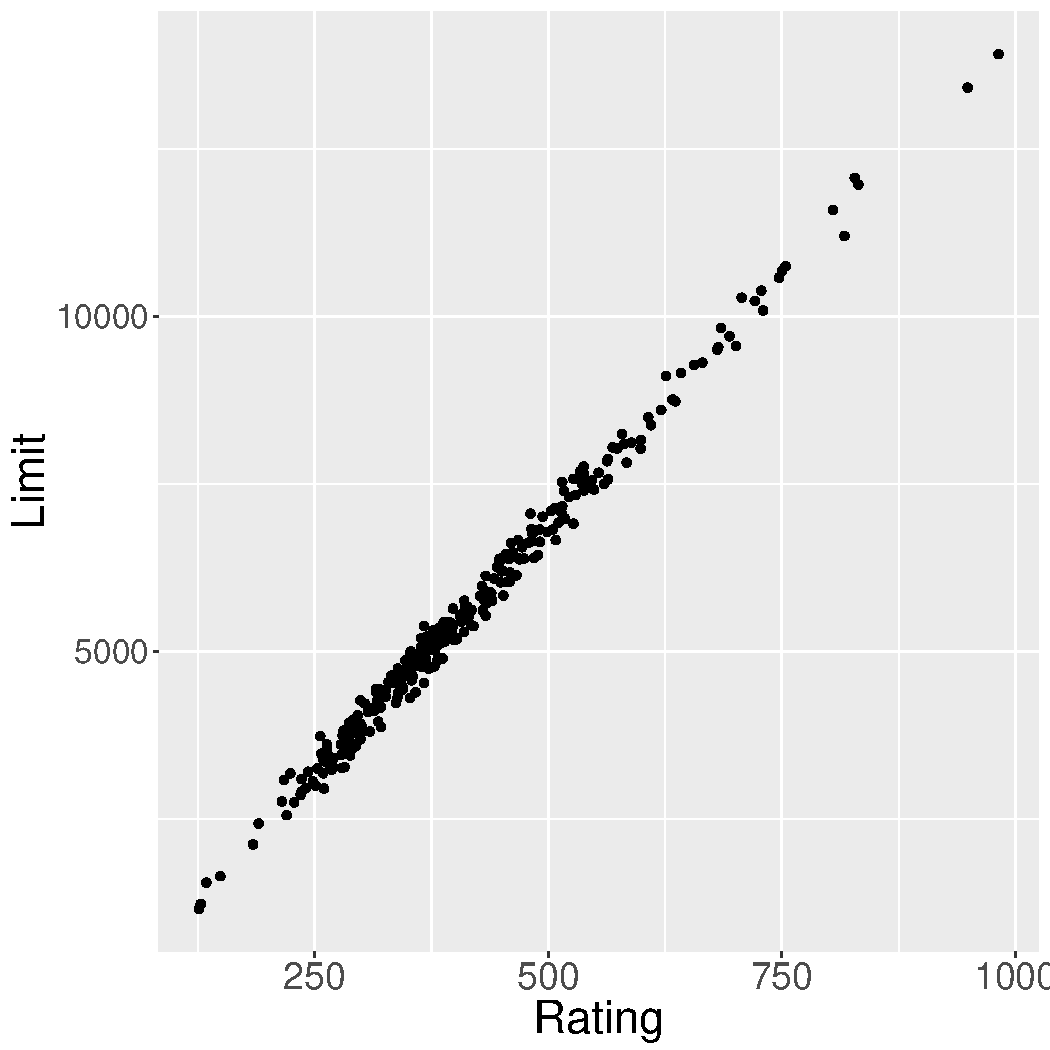
\includegraphics[scale=.3]{limitRating.pdf}
\caption{Credit limit and rating are highly collinear. }
\label{lr}
\end{figure}

One concern in our data is shown in Figure \ref{lr}. Credit rating and credit limit are highly correlated, so much so that it is reasonable to infer that credit limits are assigned based solely off rating. It is likely unnecessary to include both variables in our model since they contain the same information, and unwise because they will cause instability in our parameter estimation.


\begin{figure}
\centering
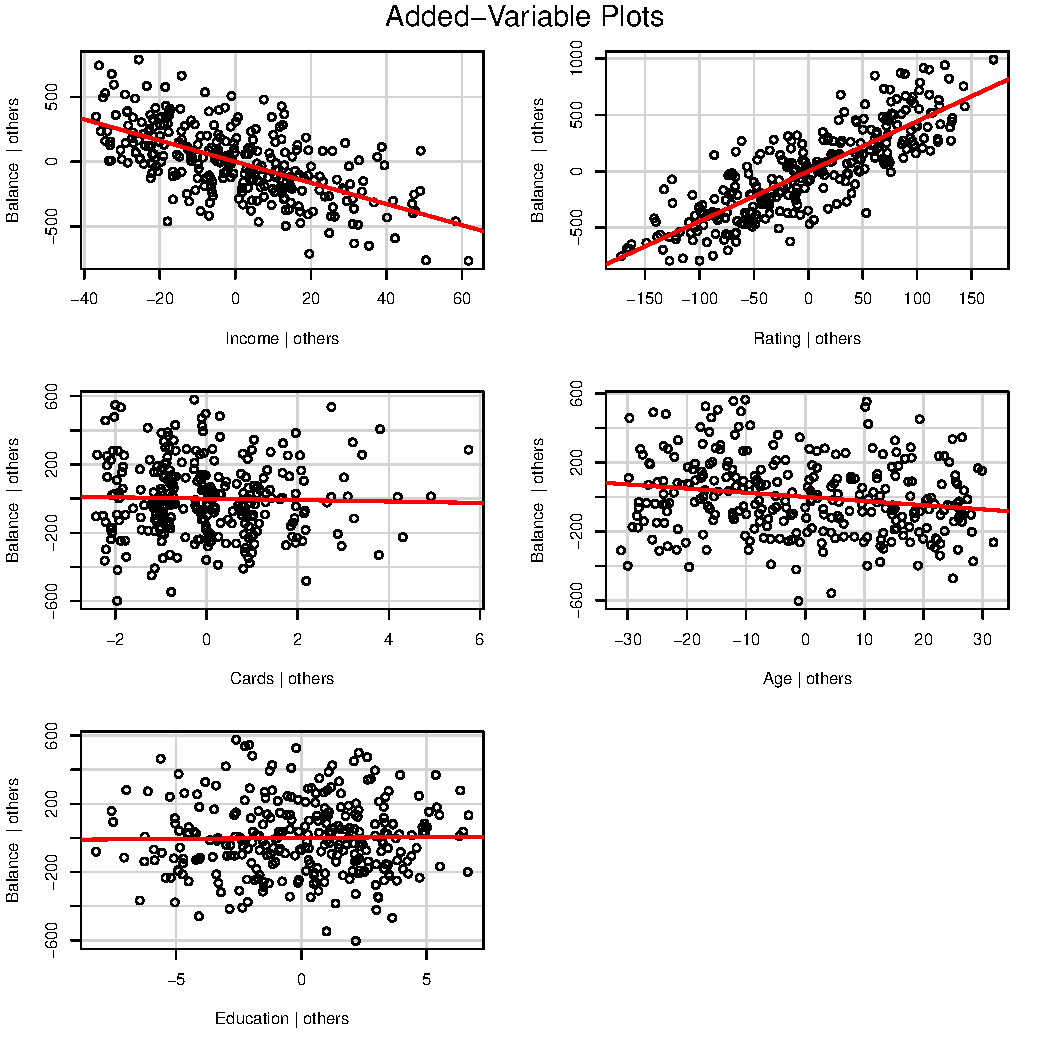
\includegraphics[scale=.5]{AVPlot.pdf}
\caption{Added variable plots for all quantitative variables. }
\label{av}
\end{figure}

The added-variable plots in Figure \ref{av} help validate our model assumptions as well as show which variables have the strongest relationship with monthly balance. The plots were created using all variables except credit limit in order to capture the true effect of credit rating. All the plots show that the linearity assumption for the relationship between the explanatory variable and the response is well justified. In addition, we don't see strong evidence of heteroskedastic data (data in which the variance is different based on the magnitude of the explanatory variable).  
\section{Model Selection}
In order to get the best confidence intervals on our effect sizes, we wanted to eliminate any spurious variables that did not inform us about our response variable. In order to see which variables did not contribute to a predictive model, we ran a AIC variable selection algorithm. Because we only have ten explanatory variables, we performed an exhaustive search for the best subset selection. 

That algorithm left us with five of our ten variables: income, limit, number of credit cards, age, and student status. A reasonable hypothesis would be that there is an interaction between income and student status. This would imply the slope for the effect of income is different if the person is a student. 

\begin{figure}
\centering
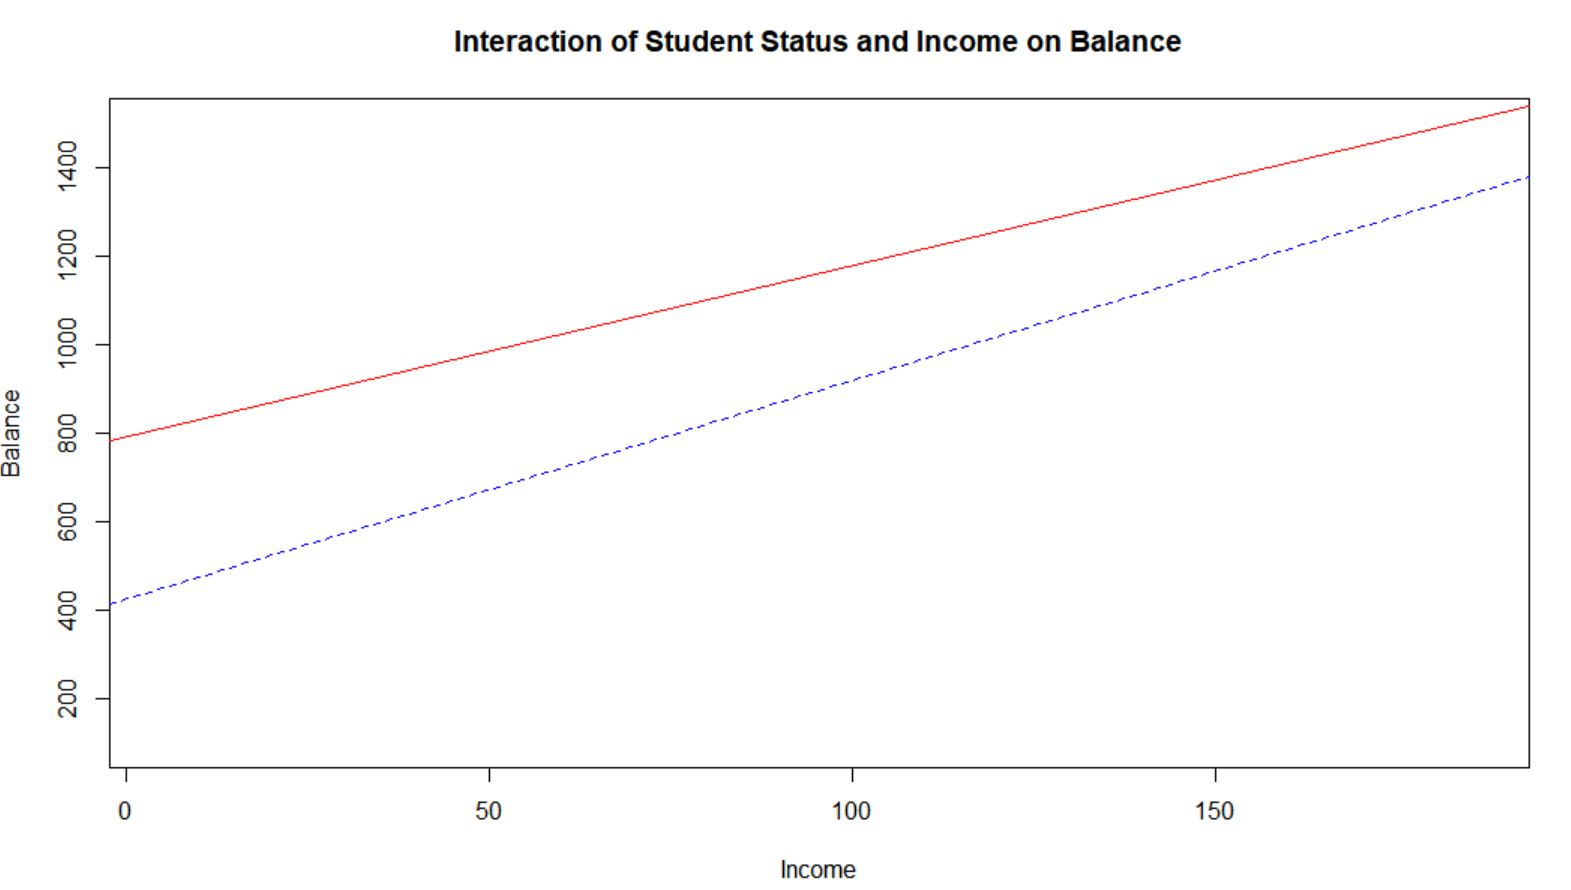
\includegraphics[scale=.7]{interaction.JPG}
\caption{Interaction Plot}
\label{interaction}
\end{figure}

Looking at the interaction plot in Figure \ref{interaction} we can see that the effect of Income on Balance is effected by the Student variable. However the lines never cross within the relevant domain of the data so the interaction does not seem very serious. However, we will test the interaction by using a more precise method. We can add this model and look at the size of the estimated effect as well as its effect on AIC. Doing this we find that our AIC goes up by almost two and the slope difference is almost 0 (0.14 with a standard error of 0.98). Therefore we will proceed without the interaction.

Our final model can be written as:

\begin{equation}
Balance = \beta_0+ \beta_1 * Income + \beta_2 * Limit + \beta_3 * Cards + \beta_4 * Age +\beta_5*Student +\epsilon
\end{equation}
$$\epsilon \sim N(0, \sigma^2)
$$          

Where $\beta_0$ is our intercept, the other $\beta$s are the effects for the explanatory variables, and $\epsilon$ are the residual errors.
\begin{figure}
\centering
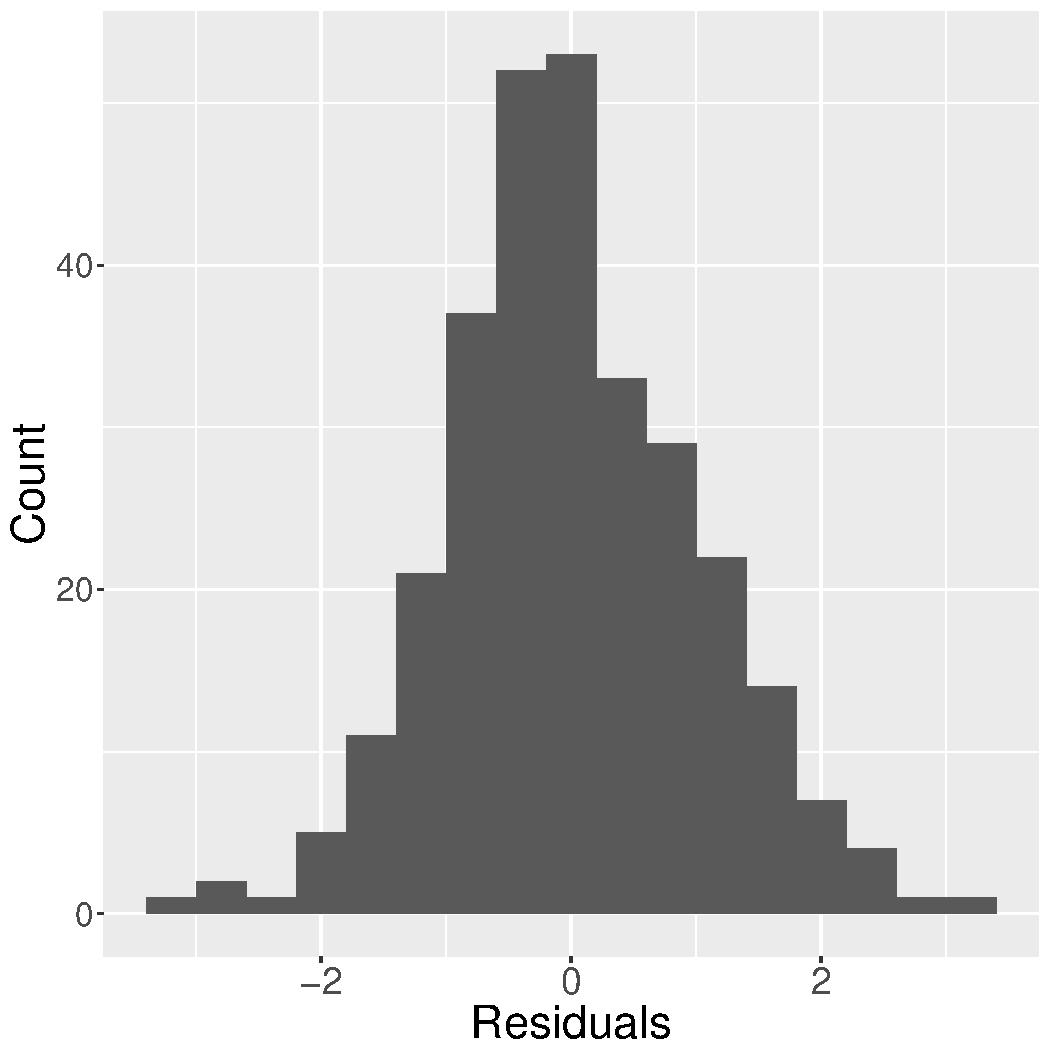
\includegraphics[scale=.3]{resids.pdf}
\caption{Errors are normally distributed}
\label{resid}
\end{figure}

Before we create predictions and confidence intervals, we can check that our assumptions are met by examining the model. Figure \ref{resid} shows standardized errors from our predictions. Our normal assumptions seems to fit the data quite well. Figure \ref{fitted} helps verify that we have homoskedastic data for all observations.  

\begin{figure}
\centering
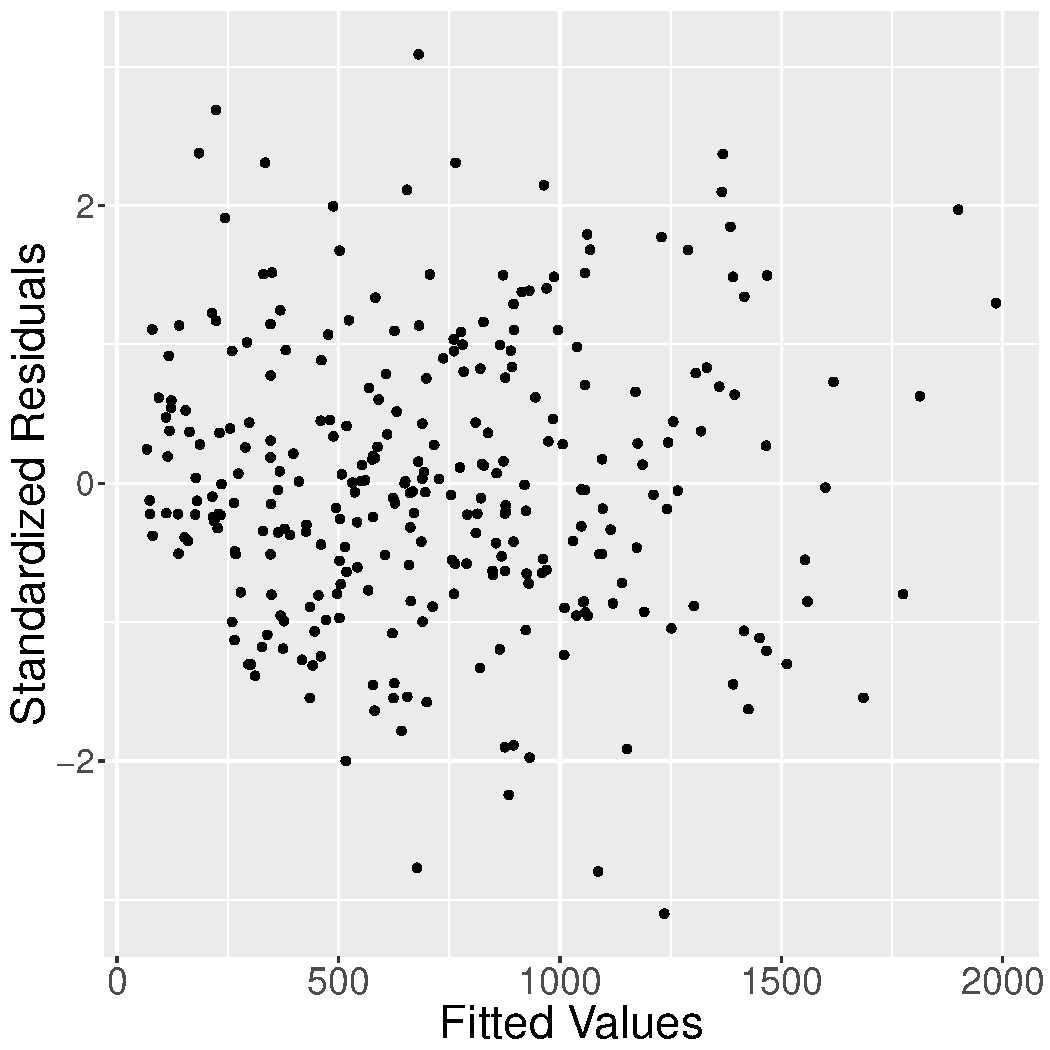
\includegraphics[scale=.3]{fitted.pdf}
\caption{Residuals don't show any distinct patterns}
\label{fitted}
\end{figure}


\begin{table}[ht]
\centering
\begin{tabular}{rrrr}
  \hline
 & Estimate & 95\% LowerBound & 95\% UpperBound \\ 
  \hline
Intercept & -527.73 & -666.55 & -388.91 \\ 
  Income & -8.55 & -9.90 & -7.20 \\ 
  Limit & 0.30 & 0.28 & 0.33 \\ 
  Cards & 18.14 & -0.87 & 37.16 \\ 
  Age & -2.59 & -4.25 & -0.94 \\ 
  Student & 511.57 & 427.10 & 596.03 \\ 
   \hline
\end{tabular}
\caption{Model Coefficient Estimates} 
\label{coefs}
\end{table}

Table \ref{coefs} shows the estimated coefficients for our linear regression model. The interpretation of each follows. We are 95\% confident that a card candidate with an income of 0, credit limit of 0, 0 other credit cards, an age of 0, and who is not a student would have credit balance between \$-666.55 and \$-388.91. We are 95\% confident that as a person's income increases by one hundred dollars, their credit card balance decreases by \$9.90 and \$7.20 on average.  We are 95\% confident that as a person's credit limit increases by one, their credit card balance increases by \$0.28 and \$0.33 on average.  We are 95\% confident that as the number other credit cards a candidate holds increases by one, their credit card balance increases by \$-0.87 and \$37.16 on average. We are 95\% confident that as the age of a candidate increases by one, their credit card balance decreases by \$4.25 and \$0.94 on average. We are 95\% confident that a candidate who is a student, has higher credit card balance than non-students by about \$427.10 and \$596.03 on average.

\section{Model Accuracy}
After fitting our model we tested the resulting model's fit through k-fold cross validation with a k of 5. We randomized the data, split into 5 folds and sequentially used each fold as a hold out set to test accuracy while we fitted the model to the other 4 folds. Our average accuracy results are included in table \ref{acc}.

\vspace{10 pt}
\begin{table}[ht]
\centering
\begin{tabular}{rr}
  \hline
  Bias &  0.33 \\ 
  RPMSE & \$213.24 \\ 
  Coverage & 94.56\% \\ 
   \hline
\end{tabular}
\caption{Model Accuracy} 
\label{acc}
\end{table}
\vspace{7 pt}

Our bias of 0.33 indicates that on average our credit card balance predictions were just 33 cents higher than the actual amounts. Our Root Predictive Mean Square Error (RPMSE) of \$213.24 indicates that our predictions were off by \$213.24 on average. Raw error values by themselves don't hold much information on model performance unless compared with other models. But the standard deviation of credit card balance in the dataset was \$450.12, so our predictions were on average less than half a standard deviation from the actual values. A metric that does hold a lot of information in model performance is that of prediction interval coverage. Our prediction interval coverage as shown in Table \ref{acc} was 94.56\%. This shows us first that our model assumptions were met very well, and second that the our model was a very good fit and was able to capture 95\% of the actual credit card balances within calculated prediction intervals.

According to the results of our cross validation, it would seem that our regression model would be able to perform well predicting credit card balances for candidates. The model could be used to predict whether or not credit card candidate should receive a card. Credit card companies would first have to establish a threshold where below a certain predicted balance no candidates would qualify for a card. But once a threshold is found, the model would be easy and accurate to use for credit card companies.

\section{Conclusion}
In this analysis we were able to show how our multiple linear regression model met the necessary assumptions for the data given and could be used for predicting credit card balance for potential credit card customers. Our model was simple and only used a few features from the original data, but proved powerful and effective. A credit card company could use the model to protect itself against bad debt from high risk customers and the company would also be able to explain why a candidate might not qualify for a card thanks to the very high interpretability of the model.

A shortcoming of our regression approach could be its exploration of interactions. Some of the variables we threw out as not meaningful may only have an effect as a two or three way interaction. Tree based methods do a better job of exploring all possible interactions. The next step in this analysis would be to gather data so as to build a model that is more robust in its prediction of unseen data. There could be a possibility that our model has too much uncertainty and that the credit card company would want more precise predictions. Gathering more data and adding more explanatory variables would allow for more precise predictions by reducing the prediction variance of the model while also keeping the interpretability of the model. 








\end{document}